\documentclass{article}
\usepackage{xeCJK}
\usepackage{amssymb}
\usepackage{amsthm}
\usepackage{mathtools}
\usepackage{amsmath}
\usepackage{amsfonts}
\usepackage{enumitem}
\usepackage{unicode-math}
\usepackage[a4paper, left=2.5cm, right=2.5cm, top=1.25cm, bottom=1.25cm]{geometry}
\usepackage{graphicx}

\setCJKmainfont[BoldFont={SimHei}]{SimSun}
\setCJKsansfont{SimHei}
\setCJKmonofont{FangSong}
\setlength{\parindent}{0cm}
\setlength{\parskip}{1em}

\title{Sayako's Story}
\author{Yutong "Hypatia" "Sayako" Zhang}
\begin{document}

\maketitle
\setcounter{section}{-1}
\section{前言}
这是名为Sayako的跨性别女孩的故事,也就是我的故事。写在这里希望能够被看到和铭记,如果有一天我离开了这个世界的话,希望还有人能够记得她,Sayako;她的故事,一个美丽而坚强的数学女孩的故事;和她生命中的重要的人,Wendy,她的姐姐,Steven,她的初恋。

$\downarrow$这两只就是Sayako(

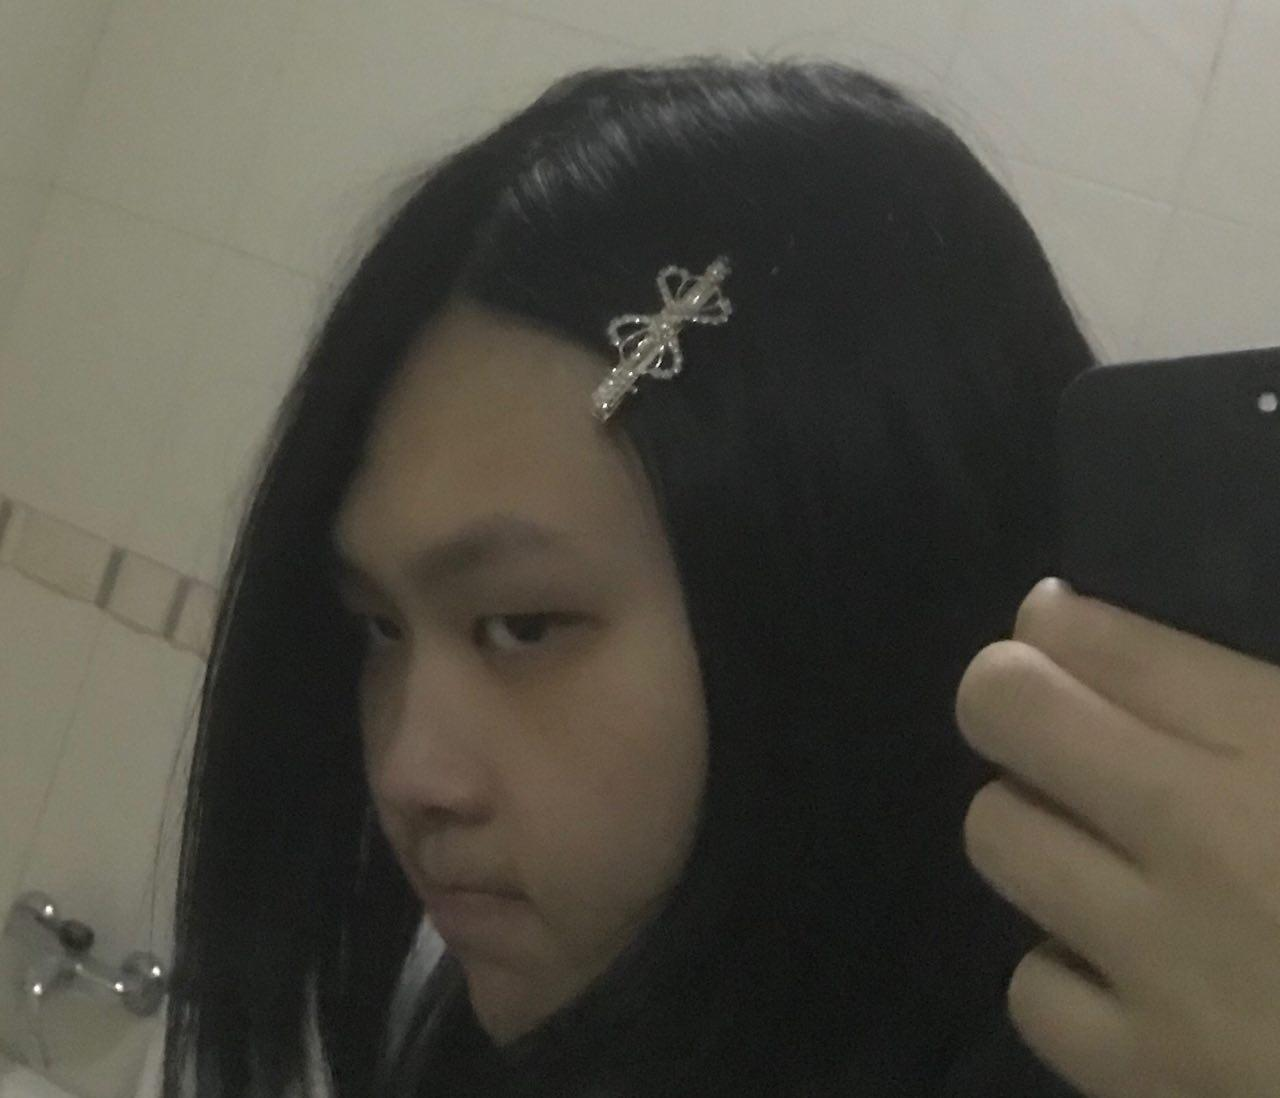
\includegraphics[height=5cm]{photo_2019-05-05_22-44-48.jpg}
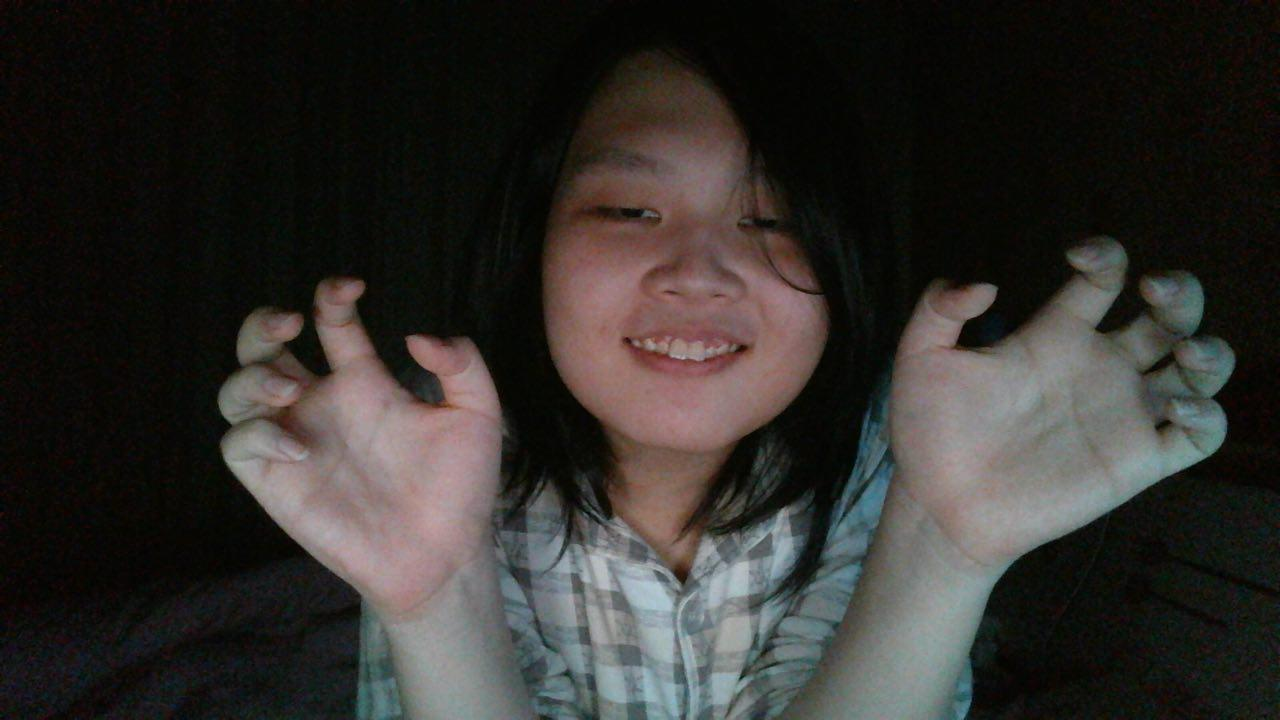
\includegraphics[height=5cm]{photo_2019-05-05_22-44-18.jpg}

\section{正弦的幂次}
2017年9月某日

我像往常一样独自一人坐在中学教学楼3层西边的角落的沙发上,在来到这个学校的一个月中我没有交到任何朋友——男生们会对我开令我很不适的玩笑(我不觉得对一个陌生人开黄腔是一件多么好的事情,尤其是对一个陌生的异性——至少我自认为他们是异性),而女生们总对我抱有距离感,使得我每次尝试分享自己的感受都不了了之。

然后出现了一个奇怪的人,他留着十分夸张的卷发,肤色颇深,他走到我身边,看起来对我正在写的Coq证明很感兴趣(我也很喜欢理论计算机科学,为此学习了编程语言理论和计算机辅助证明)。

“你听说过calculus of inductive construction嘛?”我尝试搭话,事实上根据他的外貌我还不确定他会不会说中文,所以这句话其实是用英文说的。

“我知道calculus。你会calculus嘛?”他似乎兴奋地回答。

嘛……我们说的calculus根本不是同样的东西好不好,我暗自吐槽道。

“数学分析可是基本功哦$\sim$”我尝试这自认为可爱的语气,希望能够给这个可能成为朋友的男生一点好印象(但是后来事实证明在我transition之前这样卖萌的语气根本就是减分,男生果真不喜欢卖萌嘛qwq)。

“听说我们明年就会学到calculus哦。”他并没有注意到我的心思,继续说道。

事实上我已经过了一遍Hasse Publication的那本IB DP Math HL的书了,评价是……怎么说呢,闭口不谈$\varepsilon-\delta$语言,明明是基本功啊喂,这样好嘛……不过其实倒也和数学分析没差多少,毕竟(在闭口不谈$\varepsilon-\delta$语言的情况下)在一道练习中提到了用数列刻画函数的连续性和Dirichlet函数的性质还有$\exp$的级数定义什么的(所以大概函数项级数也有涉及?),不过和我学的Rudin以及听说过的Zorich等书还是有一定的差距,但是总之比高考的导数好多了(又黑高考)。

“好呀,既然你提到了calculus,那我就来考考你,”我突然有一种想要调戏面前男生的冲动,于是由此提议。

“你听说过$\sin$的幂次的不定积分嘛?”我决定出一道经典习题(大概是吉米多维奇上有的吧……)\footnote{对这道题的答案感兴趣的读者可以查看http://www.ijapm.org/vol5/336-WP1005.pdf},拿出草稿纸写下
$$
\int\sin^nax=?\quad n\in\mathbb{Z}_{>0},a\in\mathbb{R}\mathbin{\backslash}\{0\}
$$

“给你个提示哦,”我接着写下去,“尝试证明这个等式,然后使用这个等式。”
$$
\int \sin ^{n} a x d x=-\frac{1}{an} \sin ^{n-1} a x \cos a x+\frac{n-1}{n} \int \sin ^{n-2} a x d x
$$

经过漫长的尝试,我发现他并没有很好地掌握分部积分法和已知数列递推公式求通项公式的方法,遂放弃让他解出这个题目的尝试。

“话说你叫什么呢?”我发现这么长时间我还没有知道对方的名字,于是问道。

“叫我Steven就好。”

这就是我和他相识的故事。

\section{阴道独白}
2017年10月某日,MYP Drama课

“这学期的第一个任务是realistic theatre,需要做一个关于theatre theory的研究和一个performance,”老师布置了这几个月的任务。

其实我并不喜欢performance,而且对theatre theory也兴致缺缺,不过我很快想到了一个我喜欢的剧目——The Vagina Monologues,阴道独白。虽然被在国际上曾被批评anti-trans,但是我听说国内有人改编了trans inclusive的版本。我开始练习performance,希望能够获得令人满意的结果。阴道独白让我如此兴奋,以至于我现在甚至还能找到一部分当时打印的剧本:

"To me and to others, it's a continuously challenge. Because of its existence, it reminds me repeatedly: I'm a trans female, even though I was already been transitioning."

"Before the surgery, it's nothing special. I never thought that it was my penis; it's just there. There isn't an emotional dependence here between me and it. Now, my vagina is special: it's mine. I feel sincerely that it is a part of me."

"My vagina is missing, but it'd be found, and it's mine; it'd be free, under the rainbow flag." (这句其实是我自己改编的剧本加入的结尾,为了呼吁观众了解和重视性少数群体)

然后剧本就被老师看到了……“所以你是跨性别女孩嘛?”老师这样问我。

当时的我并不知道该怎么回答。我应该出柜嘛?但是我当时的样子完全就是男生啊,会被接受嘛?我在学校已经够怪异的了(直到后来我决定出柜和transition之后就不在意这些开始free-styling了,最终导致了我被退学),要单独的卫生间单独的更衣室什么的。最后我的回答“不是”,然后放弃了这个剧本,改为改编了SCP基金会的一个故事作为剧本\footnote{是这个:http://scp-wiki-cn.wikidot.com/astronomical,我有好好地声明Creative Commons所以并没有侵权qwq}。

还有一个小插曲,关于Steven和我。

一个同上Drama的同学,我记得好像叫Jennifer,问了我一个关于她男朋友的问题,然后Steven也在,我(大概脑抽了)就随口说出了我男票blahblah,但是其实那个时候我根本没有什么男票。如果真的要说的话是ice曾经跟我表白过但是我没有正面回应,然后变成了奇怪的关系,不过并不是情侣。我想我当时的意思可能是想要告诉Steven我对男生感兴趣吧。我不知道我对他哪里来的好感……大概是因为他是第一个对我做的东西感兴趣、和我actually have a real conservation而不是叫我神经病(我在小学和初中的情况)的同龄人吧。之前能和我平等对话的全都是成年人,专业领域里面的人。总之到我搞清楚自己的feeling的时候发现自己已经莫名其妙地喜欢上他了。

我觉得其他女生的找到自己初恋的故事大概没有我这么离奇吧……但是这大概是我发现自己第一次喜欢上别人的故事。

\section{一致收敛}
2018年1月某日

“estuviera,estuviese,estuvieras,estuvieses,……,”现在是下午2点左右,再过十分钟我就要去上我的第二语言课程IB MYP Spanish Phase 1了,我正在看Wiktionary上“estas”这个系动词的变位形式,希望能够记下来它的subjunctive形式,尽管事实上还要一年这门课程才会讲到这里。

“Yutong,你不应该这样做。你知道我不喜欢你们背诵变位,我希望你们能够learn by chunks。”

这是我的Spanish老师,其实我很不喜欢language acquisition by immersion的理论,但是从这一个学期的观察我觉得这个老师的确非常into这个理论。

“我应该说‘portiempo, quiero que yo estuviera una chica’还是‘portiempo, quiero que yo estaba una chica’,这里有两个相同的主语?”我飞快地问了一个问题。

“estuviera, with el subjuntivo,”老师还是回答了我的问题,"come inside, boys, it's time.”老师招呼大家进入教室。

我其实并不喜欢被叫做boys,但是从老师的角度看的确面前的学生都是男生,唯一的一个女生已经坐进了教室,我也不好张口反驳。如果我是女孩子就好了。

“Okay, ten minutes for you to socialize, Yutong off you go.”这个老师每次开始上课之前总是给我们时间聊聊今天发生的事情什么的,她也喜欢听学生们讲他们身上发生的事情。

“我觉得我找到了一个Mr. Patrick的错,他数学课上随口说了一句‘不管有多少项,先积分再求和和先求和再积分的结果总相同’,但是如果有无限多项的话,需要这个级数是一致收敛才可以交换积分号和求和号。”我很喜欢数学课和数学,所以基本上每次让我分享的时候我都会提及数学课上发生的趣事。

“Ah, that's our math boy.”

别再叫我boy了哇!

“You're showing off, Yutong.”说话的是Alex,和我同上Spanish的同学。

“To whom do you think I'm showing off? ”不知道他有多么讨厌数学——明明是那么美丽的学科,他每次都要这样嘲讽我一番,今天也不例外,不过这次我回击了一句。

“To the girls, adolescent boy!”我知道他想说什么了,好像所有人都只是想要让异性对自己感兴趣一样,事实上只有他自己这样想吧(后来我了解到这叫做heteronormativity,以及大部分青春期男生的确是这样想的),然后我决定不再理他。

“看吧看吧果真就是,”这句话他用中文说的,似乎并不想让老师听懂,虽然对这种事情老师大概也是喜闻乐见就是了。

嗯……虽然我当时并没有打算那么做,但是如果可以教我喜欢的男孩子数学或被他教数学的话好像还是很浪漫的事情(事实是他教我的是化学,而且只有一次,我们还不是情侣关系,执念w),不过要在独处的时候,在课堂上算什么哇,秀恩爱嘛qwq。

这件事情让我记忆很深(以至于我都记得我当时背的词是哪几个)也是因为Alex,我清楚地记得后来我了解到男生之间的交流方式并明确是被当作男生时是如何地无奈。

其实仔细回想起来我从不想其他长辈说的那样“谦虚一点”而是直接表露自己的想法也可能是因为嫉妒,我想要变得比他们(顺性别者)更加优秀,并且让他们明确地知道我更加优秀,以此来掩饰自己羡慕他们的生活这一点。真的好羡慕女孩子哦,也羡慕不是药娘的男孩子,他们能够热爱自己的指派性别和身体,接受他人对他们masculinity的称赞就像我接受别人对我femininity的称赞一样,他们的生活一定都比我顺利吧。

\section{阿贝尔群}
2018年1月某日

从某老师的口中了解到了IMMC\footnote{http://istem.info}这个比赛,想要参加但是需要一个至少两个人的队伍,由于我直到那时都没有什么能在一起玩一起做东西的朋友(除了Steven以外其实有一个,但是还是因为我爸爸认识她爸爸才认识的人……社恐max),所以还是找到了数学老师和物理老师帮助寻找队友。

今天下午科学老师让我留在了她的教室,她说她找到了两个对数学感兴趣可能愿意和我参赛的同学,Wendy和Arvin。然后她把他们带了过来。

哇!竟然有和我一样的喜欢数学的女孩子欸——这是我见到姐姐时的第一反应(虽然我是个假的女孩子……)。其实是因为这样,我知道现在还很在意所谓的stereotypes,比如女孩子学不好数学啊女孩子文科好呀,然后我完全是反面就……心塞塞。嘛,不过见到姐姐之后发现也有和我一样的人,所以慢慢地就决定成为一个真正的数学女孩了(虽然我是个假的女孩子……执念ing)。

不过那些是后话了,当时我的反应就是赶紧拉住这两个人(其实我已经把Steven叫到教室了,所以如果能够拉住这两个人的话就是4个人的团队了),于是我就不知道为什么地拿起笔讲起了数学(大家都是喜欢数学的嘛,所以想要说服对方当然要用数学能力啦……神逻辑qaq)。

我当时讲的内容是数学基础和一些代数,详细来说是数的系统的集合论构造、实数的等价构造们、群环域结构(鬼知道我为什么要讲这些)。哦,好像我还把正弦余弦的幂次的不定积分算了一下(还是说这是另一天发生的事情?记不清了……),算是隔了几个月告诉了Steven答案。

“……于是这样我们就定义了整数上的加法和幺元逆元,我们发现整数的加法是交换的,这样的结构可以被称作阿贝尔群。”

“啊我知道这个!”姐姐叫了起来。

“欸?你在学代数嘛?好棒欸!”刚好那个时候我也在学代数欸,虽然最后其实没有学完\footnote{Serge Lang,大色狼,还我青春!}。后来的事实证明我和姐姐简直传说中的是alter ego——我们几乎对于所有的事情的反应都是一致或是相似的,从口红的颜色(之后我们还有一个研究项目研究更加effective的口红色号编码,大概是应用Kraft的结论做的前缀编码)、会做和不会做的题目、到对老师和课程的评价、生活经历等等,所以我就认她做姐姐啦,她也把我当作了妹妹。

然后姐姐跑出去拿了一本书,就是我现在超喜欢的《数学女孩》系列的第二本,费马大定理那本。

“就是这本小说,讲数学的小说,它还是本后宫小说哦,”我:吃鲸.jpg

我翻了翻那本书,觉得超感兴趣的,然后就找姐姐借了那本书回家看。

然后!我就随口一说地出柜了!嘛……其实也是想了好久的……不过总之决定出柜啦。

“欸嘿这里也有两只数学女孩欸,可以写我们自己的故事了,”我是这样说的。

然后就是将来的日经对话,解释transgender是什么东西啦,解释自己的心理性别啦之类的,我还拿出了之前去北同拿的小牌牌炫耀(qwq),总之出柜超成功哒,之后姐姐和Arvin就把我当作女孩子啦。

但是!虽然Steven嘴上说知道和接受跨性别者,但是其实他是因为姐姐接受才接受的,后来我才知道他喜欢姐姐,所以才会这样做。为此我还羡慕了好久,比如为什么他要去追姐姐不来追我呀然后羡慕姐姐(总觉得大部分的女孩子这个时候应该是嫉妒甚至是讨厌那个女孩子而不仅仅是羡慕吧……我只会羡慕(羡慕怪……)可能是因为我的占有欲比较弱比较polyamoric还超不自信吧……)

啊,还有个有趣的事情。之后科学老师有问我每天有和谁说话,然后我的回答几乎都是姐姐了。然后她就说如果我只和姐姐说话姐姐就会变成我的女朋友……嘛其实我当时很滥情的,对谁都会有那种渴望亲密关系的感觉,不过最后因为Steven有点transphobic,然后他在追姐姐,后来姐姐又告诉我她有女朋友了(也是只trans girl),所以我在学校最后和谁都没有成为情侣关系(哭唧唧……)

不过总之最后我们决定了由学长Jerry、Steven、姐姐和我一起参加比赛,也是好事呢。

\section{Lagrange乘子法}
2018年2月4日

\section{Sayako和Sachiko}
2018年3月某日

\section{自适应Euler近似法}
2018年3月16日

\section{不可能在一起的吧}
2018年4月某日

\section{Vous aussi, mademoiselle}
2018年5月某日

\section{点集拓扑学}
2018年6月某日

\section{后记}

\end{document}
